%==============================================================================
% ETHASL - Template for student projects at the ASL
% 2013.10: Péter Fankhauser
% This template is based on the IMRT Latex template by Eric A. Mueller.
%==============================================================================

\documentclass[10pt,twoside,a4paper]{report}

% ETHASL package
% TODO Choose options according to your project
% som/bt/st/mt: Studies on Mechatronics, Bachelor Thesis, Semester Thesis, Master Thesis
% fs/hs: Spring term, Autumn term
% german/english: German/English

\usepackage[bt,hs,english]{packages/ethasl}
\usepackage[linesnumbered]{algorithm2e}
\usepackage[noend]{algpseudocode}
\usepackage{textcomp}
\usepackage{listings}
\renewcommand{\lstlistingname}{Code}
\definecolor{listinggray}{gray}{0.9}
\definecolor{lbcolor}{rgb}{0.9,0.9,0.9}

%---------------------------------------CODE------------------------------------------ %%
\lstset{
	backgroundcolor=\color{lbcolor},
	tabsize=2,
	rulecolor=,
	language=C++,
	%basicstyle=\scriptsize, % noch kleinerer Code
	basicstyle=\ttfamily, %mittlerer Code
	upquote=true,
	%aboveskip={1.5\baselineskip},
	columns=fixed,
	showstringspaces=false,
	extendedchars=true,
	breaklines=true,
	prebreak = \raisebox{0ex}[0ex][0ex]{\ensuremath{\hookleftarrow}},
	frame=single,
	showtabs=false,
	showspaces=false,
	showstringspaces=false,
	identifierstyle=\ttfamily,
	keywordstyle=\color[rgb]{0,0,1},
	commentstyle=\color[rgb]{0.133,0.545,0.133},
	stringstyle=\color[rgb]{0.627,0.126,0.941},
	numbers=left,
	numberstyle=\tiny,
	stepnumber=1,
	numbersep=5pt
}
%----------------------------------------------------------------------------------------- %%

%\usepackage{algorithm}
%\usepackage{algorithmic}

% Activate for german language
%\usepackage{german}
%\usepackage{ae}

%\documentclass{article}
%\usepackage{algorithm,algcompatible,amsmath}
%\DeclareMathOperator*{\argmax}{\arg\!\max}% http://tex.stackexchange.com/q/83169/5764
%\algnewcommand\INPUT{\item[\textbf{Input:}]}%
%\algnewcommand\OUTPUT{\item[\textbf{Output:}]}%


%\usepackage{algorithm2e}% http://ctan.org/pkg/algorithm2e
%\makeatletter
%\renewcommand{\@algocf@capt@plain}{above}% formerly {bottom}
%\makeatother

%%%%%%%%%%%%%%%%%%%%%%%%%%%%%%%%%%%%%%%%%%%%%%%%%%%%%%%%%%%%%%%%%%%%%%%%%%%%%%%
% LaTeX preamble
%%%%%%%%%%%%%%%%%%%%%%%%%%%%%%%%%%%%%%%%%%%%%%%%%%%%%%%%%%%%%%%%%%%%%%%%%%%%%%%
% Encoding settings
\usepackage[utf8]{inputenc}
\usepackage[OT1]{fontenc}

% Paper size
\usepackage{a4}

% Headings
\usepackage{fancyhdr}

% More symbols
\usepackage{textcomp}\usepackage{gensymb}

% Math support for Times font
%\usepackage{txfonts}

% ISO date
\usepackage[english]{isodate}

% Multi column
\usepackage{multicol}

% Figures
\usepackage{graphicx}

% Subfigures (obsolete)
\usepackage{subfigure}

% Bibliography
\usepackage[numbers]{natbib}

% Nicer tables
\usepackage{booktabs}
\usepackage{array}
\usepackage{multirow}

% Colors
\usepackage{color}
\usepackage{colortbl}
\definecolor{black}{rgb}{0,0,0}
\definecolor{white}{rgb}{1,1,1}
\definecolor{darkred}{rgb}{0.5,0,0}
\definecolor{darkgreen}{rgb}{0,0.5,0}
\definecolor{darkblue}{rgb}{0,0,0.5}

% Additional math functionality
\usepackage{amsmath}
\usepackage{amssymb}

% Nice fractions
\usepackage{nicefrac}

% Upper case greek letters
\usepackage{upgreek}

% ISO math notation
\usepackage{isomath}
\renewcommand{\vec}{\vectorsym}
\newcommand{\mat}{\matrixsym}

% Units
\usepackage{units}

% Rotated objects
\usepackage{rotating}

% Indent
\setlength{\parindent}{0em}

% Include PDF pages
\usepackage{pdfpages}
\includepdfset{pages={-}, frame=true, pagecommand={\thispagestyle{fancy}}}

% Headings
\rhead[\thepage]{\nouppercase{\rightmark}}
\lhead[\nouppercase{\leftmark}]{\thepage}
\cfoot{}

% Gantt chart
\usepackage{pgfgantt}

% Links (last package)
\PassOptionsToPackage{hyphens}{url}\usepackage{hyperref}

% Clever references (has to be loaded after hyperref)
\usepackage{cleveref}


%%%%%%%%%%%%%%%%%%%%%%%%%%%%%%%%%%%%%%%%%%%%%%%%%%%%%%%%%%%%%%%%%%%%%%%%%%%%%%%
% Title page
%%%%%%%%%%%%%%%%%%%%%%%%%%%%%%%%%%%%%%%%%%%%%%%%%%%%%%%%%%%%%%%%%%%%%%%%%%%%%%%
\begin{document}

% TODO Add your title
\title{Path Planning for an Omnidirectional Underwater Robot}
%\subtitle{bla bla bla}

% TODO Add name of the authors
\studentA{Johann Diep}
%\studentB{Student 2}
% \studentC{Student 3}

% TODO Add name of the supervisors
\supervisionA{Gregory Hitz}
\supervisionB{Philipp Krüsi}
%\supervisionC{Supervisor C}

% TODO Change if necessary
\projectYear{\the\year} % This year
%\projectYear{\advance\year by -1 \the\year\advance\year by 1} % Last year

\maketitle
\pagestyle{plain}
\pagenumbering{roman}

%%%%%%%%%%%%%%%%%%%%%%%%%%%%%%%%%%%%%%%%%%%%%%%%%%%%%%%%%%%%%%%%%%%%%%%%%%%%%%%
% Declaration of originality
%%%%%%%%%%%%%%%%%%%%%%%%%%%%%%%%%%%%%%%%%%%%%%%%%%%%%%%%%%%%%%%%%%%%%%%%%%%%%%%
\pagestyle{empty}

% TODO Modify placeholders in declaration.tex
% TODO Add title, student first/last name, supervisor first/last name.

\section*{Declaration of Originality}

\vspace{1cm}

I hereby declare that the written work I have submitted entitled

\vspace{0.5cm}

% TODO Add title
\textbf{Your Project Title}

\vspace{0.5cm}

is original work which I alone have authored and which is written in my own words.\footnote{Co-authored work: The signatures of all authors are required. Each signature attests to the originality of the entire piece of written work in its final form.}

\vspace{1cm}

\textbf{Author(s)}

\vspace{0.5cm}

\begin{tabular}{ p{5cm} p{5cm} }
% TODO Add student first/last name
  Johann & Diep \\
\end{tabular}

\vspace{0.5cm}

\textbf{Student supervisor(s)}

\vspace{0.5cm}

\begin{tabular}{ p{5cm} p{5cm} }
% TODO Add supervisor first/last name
  Gregory & Hitz \\
  Philipp & Kr\"usi \\
\end{tabular}

\vspace{0.5cm}

\textbf{Supervising lecturer}

\vspace{0.5cm}

\begin{tabular}{ p{5cm} p{5cm} }
  Roland & Siegwart \\
\end{tabular}

\vspace{1cm}

With the signature I declare that I have been informed regarding normal academic citation rules and that I have read and understood the information on 'Citation etiquette' (\url{https://www.ethz.ch/content/dam/ethz/main/education/rechtliches-abschluesse/leistungskontrollen/plagiarism-citationetiquette.pdf}).
The citation conventions usual to the discipline in question here have been respected.

\vspace{0.5cm}

The above written work may be tested electronically for plagiarism.

\vspace{4cm}

\begin{tabular}{ p{5cm} p{1cm} p{5cm} }
  \cline{1-1} \cline{3-3}
  Place and date & & Signature \\
\end{tabular}


%%%%%%%%%%%%%%%%%%%%%%%%%%%%%%%%%%%%%%%%%%%%%%%%%%%%%%%%%%%%%%%%%%%%%%%%%%%%%%%
% Table on contents
%%%%%%%%%%%%%%%%%%%%%%%%%%%%%%%%%%%%%%%%%%%%%%%%%%%%%%%%%%%%%%%%%%%%%%%%%%%%%%%

% Table of Contents depth (TODO change if necessary)
\setcounter{tocdepth}{2}

\tableofcontents
\cleardoublepage

%%%%%%%%%%%%%%%%%%%%%%%%%%%%%%%%%%%%%%%%%%%%%%%%%%%%%%%%%%%%%%%%%%%%%%%%%%%%%%%
% Chapters standard
%%%%%%%%%%%%%%%%%%%%%%%%%%%%%%%%%%%%%%%%%%%%%%%%%%%%%%%%%%%%%%%%%%%%%%%%%%%%%%%
\chapter*{Preface}
\addcontentsline{toc}{chapter}{Preface}
%\chapter*{Vorwort}
%\addcontentsline{toc}{chapter}{Vorwort}

At this point I would like to thank everyone who supported me during this bachelor thesis. First of all, I would like to express my gratitude to Professor Dr. Roland Siegwart and the \textsc{Autonomous Systems Lab} (ASL) for their continuous support of the focus project \textsc{Scubo}. Special thanks to my supervisors Dr. Gregory Hitz and Philipp Kr\"usi for guiding me successfully throughout the whole project. Last but not least, I would like to thank the whole \textsc{Scubo} team. It was an amazing roller coaster ride and I am very grateful to be a part of it since the very beginning. \\

Zurich, June 2016 \\

Johann Diep    
\cleardoublepage
\chapter*{Abstract}
\addcontentsline{toc}{chapter}{Abstract}
%\chapter*{Zusammenfassung}
%\addcontentsline{toc}{chapter}{Zusammenfassung}

\textsc{Scubo} is a submersible ROV (Remotely Operated Vehicle) developed in the context of a focus project at ETH Zurich. Due to the arrangement of eight non-moving propulsion units and the superposition of its forces, it is able to move in any direction without prior change of its orientation. Besides, it is equipped with six cameras pointing in each direction and the necessary hardware for autonomy. Several bachelor theses are concerned with the software implementation of an autonomous path following system. \\  

This bachelor thesis discusses the implementation of an offline global path planning algorithm for the \textsc{Scubo} robot. The algorithm uses a point cloud\footnote{A point cloud is a set of data points representing positions of features. It can be generated by post-processing recordings of a stereo camera and an IMU with a mapping software.} of the environment to generate a set of collision-free waypoints between an initial and a goal state for the trajectory controller to follow. Since the robot is capable of omnidirectional movements, the generated path does not have to satisfy any kinematic or dynamic constraints of the system other than avoiding collision with obstacles. \\

At first, the basic idea behind available path planning methods are explained on a conceptual level. In a second step, the implementation of the path planning algorithm using a variant of the rapidly-exploring random tree (RRT) method is presented in more detail. Lastly, the algorithm is used in a practical application where the goal is to scan an object from all sides under different angles. In this case, the developed path planner in combination with a traveling salesman problem solver proves to be highly suitable to generate a collision-free and cost-efficient path around an object.   



\cleardoublepage
\chapter*{Symbols}
\label{sec:symbols}
\addcontentsline{toc}{chapter}{Symbols}
%\chapter*{Symbolverzeichnis}
%\label{sec:symbole}
%\addcontentsline{toc}{chapter}{Symbolverzeichnis}

%\section*{Symbols}
%%\section*{Symbole}

%\begin{tabbing}
% \hspace*{1.6cm} \= \kill
%%  $\phi, \theta, \psi$    \> roll, pitch and yaw angle \\[0.5ex] 					
%%  $b$                     \> gyroscope bias \\[0.5ex]										
%%  $\Omega_m$              \> 3-axis gyroscope measurement \\[0.5ex]   		
%\end{tabbing}

%\section*{Indices}
%%\section*{Indizes}
%\begin{tabbing}
% \hspace*{1.6cm}  \= \kill
%% $x$ \> x axis \\[0.5ex]
%% $y$ \> y axis \\[0.5ex]
%\end{tabbing}

\section*{Acronyms and Abbreviations}
%\section*{Akronyme und Abkürzungen}
\begin{tabbing}
 \hspace*{1.6cm}  \= \kill
 ASL \> Autonomous Systems Lab \\[0.5ex]
 ETH \> Eidgenössische Technische Hochschule \\[0.5ex]
 IMU \> Inertial Measurement Unit \\[0.5ex]
 k-d \> k-dimensional \\[0.5ex]
 LCA \> Label Correcting Algorithm \\[0.5ex]
 LKH \> Lin-Kernighan Heuristic \\[0.5ex]
 PRM \> Probabilistic Roadmap \\[0.5ex]
 ROV \> Remotely Operated Vehicle \\[0.5ex]
 RRT \> Rapidly-Exploring Random Tree \\[0.5ex] 
 RRT* \> Rapidly-Exploring Random Tree Star \\[0.5ex]
 SLAM \> Simultaneous Localization and Mapping \\[0.5ex]
 VIO \> Visual-Inertial Odometry \\[0.5ex]
 VR \> Virtual Reality \\[0.5ex]
% EKF \> Extended Kalman Filter \\[0.5ex]
% IMU \> Inertial Measurement Unit \\[0.5ex]
% UAV \> Unmanned Aerial Vehicle \\[0.5ex]
% UKF \> Unscented Kalman Filter \\[0.5ex]
\end{tabbing}
\cleardoublepage

%%%%%%%%%%%%%%%%%%%%%%%%%%%%%%%%%%%%%%%%%%%%%%%%%%%%%%%%%%%%%%%%%%%%%%%%%%%%%%%
% Chapters custom
%%%%%%%%%%%%%%%%%%%%%%%%%%%%%%%%%%%%%%%%%%%%%%%%%%%%%%%%%%%%%%%%%%%%%%%%%%%%%%%
\pagestyle{fancy}
\pagenumbering{arabic}

% TODO Add your own chapters here
\nocite{*}
\chapter{Introduction}
\label{sec:introduction}

This section gives the reader a brief overview of the motivation, the context and the scope of this bachelor thesis.

\section{Motivation}

\textsc{Scubo} is a submersible robot (see Figure ~\ref{pics:scubo_robot}) developed in the scope of a focus project at ETH Zurich. During two semester, a team consisting of mechanical and electrical engineering students had the opportunity to build a functional prototype of a robot. The goal of the project was to design a manually controlled submersible robot which is capable for 3D reconstruction of single corals. By taking pictures from different sides and angles of the underwater object, a detailed model can be obtained in post-processing by feeding these pictures to a suitable third party software like \textsc{Pix4D}\footnote{https://pix4d.com/}. This way, changes of coral reefs can be well observed and documented. Furthermore, the robot should provide telepresence for exploration of underwater landscapes. With the help of six on-board cameras, the user has access to a visual feedback from all sides of the robot through a VR-headset. The overall goal for the future is a further development of \textsc{Scubo} into a fully autonomous system. This has the following benefits:  

\begin{itemize}
	\item 
	Common image processing software is based on finding keypoints\footnote{Characteristic points detected in an image.} between images, which will generate 3D points. By increasing the overlap between two images, the common area captured is larger and more keypoints can be detected and matched together. Consequently, a rule of thumb is to maintain high overlap between the images. This can be done by keeping a constant distance while slightly varying the angle to the object. Therefore, scanning corals via remote control is difficult since the user has to control the distance as well as the orientation of the robot to the object. This task can be simplified by generating an efficient trajectory consisting of position and orientation information around that object for the autonomous system to follow.
	\item 
	One possible application of \textsc{Scubo} and its virtual reality feature is the deployment in large aquariums of entertainment parks. These are narrow environments containing static as well as dynamic obstacles such as glass walls and underwater creatures. Collision in such sensitive surroundings would endanger the safety of the audience and the animals. This problem can be prevented by an autonomous system that is able to follow a predefined collision-free path. In this way, the audience can observe the environments through a VR-headset without having to control the robot. 
\end{itemize}

\begin{figure} [h]
	\centering
	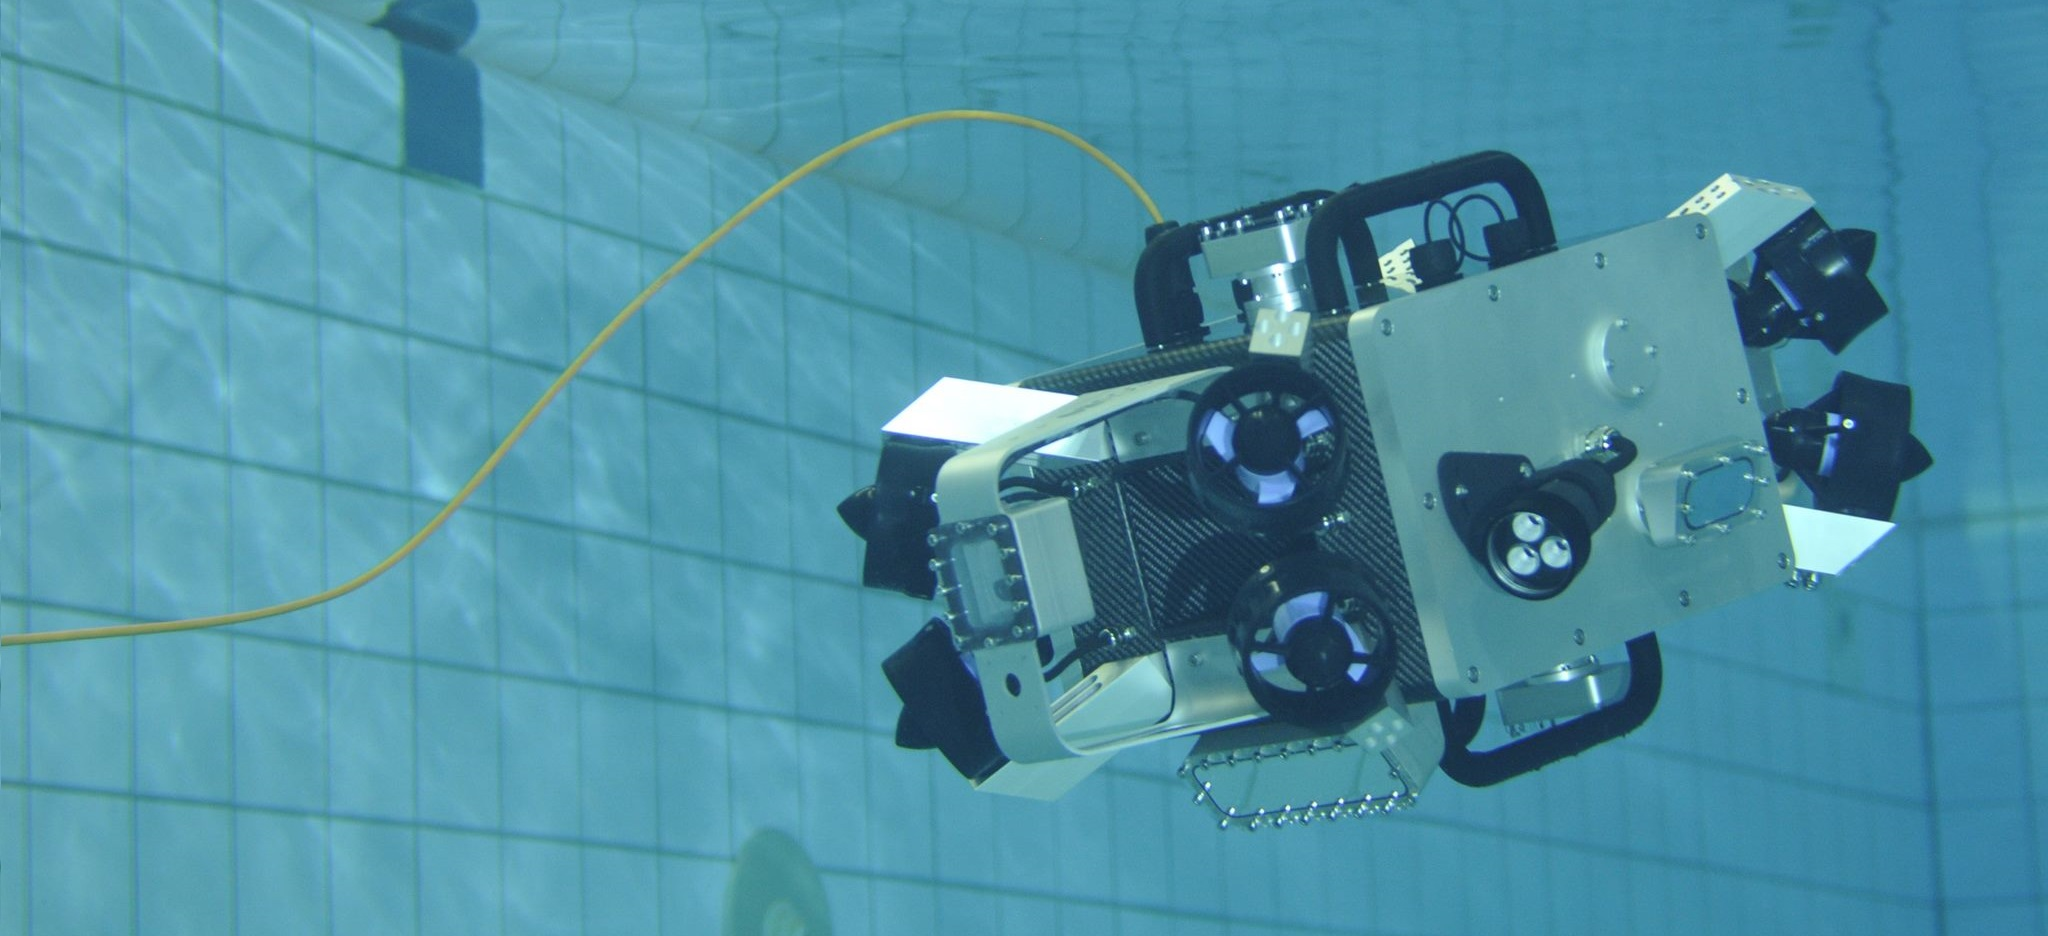
\includegraphics[width=0.9\textwidth]{images/Scubo_robot.jpg}
	\caption{The \textsc{Scubo} robot in action.}
	\label{pics:scubo_robot}
\end{figure}
  
\section{Context}  
  
This bachelor thesis discusses planning algorithm and aims to complement the work of the focus project \textsc{Scubo}. Together with several other bachelor theses, its goal is to build the foundation for an autonomous system based on computer vision. In the following an overview of the theses and their associations is given:

\begin{itemize}
	\item
	Underwater Camera Calibration: The process of determining all the necessary parameters for the image rectification in underwater application. 
	\item
	Localisation and Mapping: State estimation and 3D reconstruction of the environment to a point cloud by post-processing recordings of the calibrated stereo camera and an IMU (VIO-sensor). 
	\item
	Path Planning: Implementation of an algorithm which generates a collision-free trajectory from a starting to a destination point using the previous generated point cloud.
	\item 
	Trajectory Controller: Design of controller needed to follow the generated set of waypoints. 
\end{itemize}

\section{Goal}
The goal of this bachelor thesis is the development of an offline path planning algorithm as a basic for a semi-autonomous\footnote{The planning algorithm of a semi-autonomous system requires the complete map in advance and does not calculate the set of waypoints in real-time.} system. The designed algorithm should provide a set of global waypoints of position informations from start to finish while avoiding collision with obstacles. Furthermore, a method should be found to generate a trajectory around an object for scanning purpose. The following framework conditions apply: 

\begin{itemize}
	\item
	The visible areas by the robot is represented by a certain space called the workspace. The robot itself is represented in the workspace by its centre of mass point.  
	\item
	Obstacles in the form of a point cloud represents not accessible states.
	\item
	Starting and goal state are predefined input variables.	
\end{itemize}

	

\cleardoublepage
\chapter{Related Work }
\label{sec:related_work}

This chapter gives a brief overview of available planning methods. One distinguish between roadmap, cell decomposition, potential field, sampling-based and graph-search planning methods\footnote{A similiar classification can be found in the bachelor thesis Robotic Arm Motion Planning by Markus Br\"andle}. A detailed description can be found in (Siegwart, 2004, \cite{Siegwart2004}), (Karaman, 2011, \cite{Karaman2011}) and (Bertsekas, 1995, \cite{Bertsekas1995}).

\section{Roadmap Path Planning}

This method is based on constructing a graph network consisting of lines in the obstacle-free configuration space\footnote{Vector space defined by the generalized coordinates of a system.}. The actual planning is then reduced to connecting the initial and goal state of the robot to the network and searching for feasible paths between them. In the following, two roadmap approaches are described.

\subsection{Visibility Graph}

The visibility graph is mostly suitable and highly efficient for sparse 2D configuration spaces with polygonal obstacles. The nodes of the graph include the vertices of the obstacles as well as the initial and final point. Straight-line segments connect every nodes that are visible from each other (i.e. sight is not blocked by an obstacle), which also includes the edges of the polygons. Thus, the optimal path in terms of length between start and goal state can be found (see Figure \ref{pics:visibility_graph}). The implementation of the visibility graph is straight forward, however, there are two major drawbacks of this method. First, the computational effort increases with the number of obstacles, which lowers the efficiency of the algorithm in dense environments. Second, the algorithm tends to generate a path as close as possible to nearby obstacles. However, the latter can be solved by expanding the size of the obstacles or using another roadmap method called the Voronoi diagram. 

\begin{figure} [h]
	\centering
	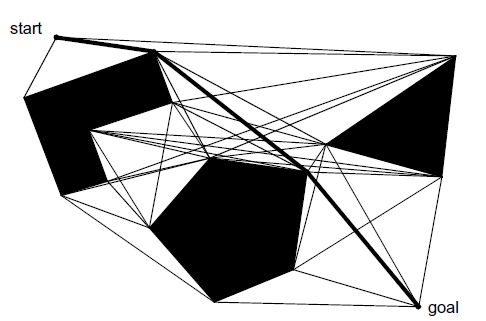
\includegraphics[width=0.5\textwidth]{images/visibility_graph.png}
	\caption{Visibility graph, 'this image is taken from \cite{Siegwart2004}'.}
	\label{pics:visibility_graph}
\end{figure}

\subsection{Voronoi Diagram}

In contrast with the visibility graph method, a Voronoi diagram (see Figure \ref{pics:voronoi_graph}) maximizes the distances between the robot and the obstacles in the configuration space (including the boundaries). It consists of equipotential line-segments constructed from points that are equidistant from two or more obstacles. 

\begin{figure} [h]
	\centering
	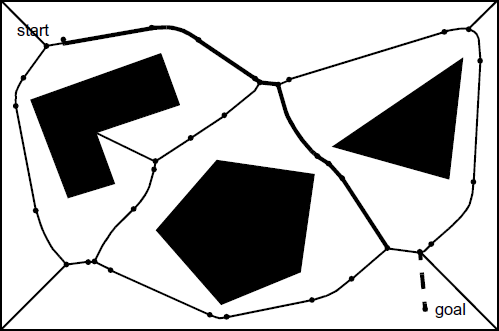
\includegraphics[width=0.5\textwidth]{images/voronoi_graph.png}
	\caption{Voronoi diagram, 'this image is taken from \cite{Siegwart2004}'.}
	\label{pics:voronoi_graph}
\end{figure}

\section{Cell Decomposition Path Planning}

The general idea of the cell decomposition method can be summarized as follows:

\begin{itemize}
	\item
	splitting of the configuration space into smaller non-overlapping regions called \textit{cells},
	\item
	constructing a \textit{connectivity graph} according to the cell-conjunctions,
	\item
	searching for a sequence in the connectivity graph that joins the initial with the goal cell,
	\item
	computation of a path passing through each cell of the sequence.
	
\end{itemize}

Depending on the cell division, one distinguish between exact and approximate cell decomposition.

\begin{itemize}
	\item
	Exact cell decomposition: Boundaries of the cells corresponds to the structure of the environment (see Figure \ref{pics:cell_decomposition}).
	\item
	Approximate cell decomposition: Division into cells results in an approximation of the map. 
\end{itemize}

\begin{figure} [h]
	\centering
	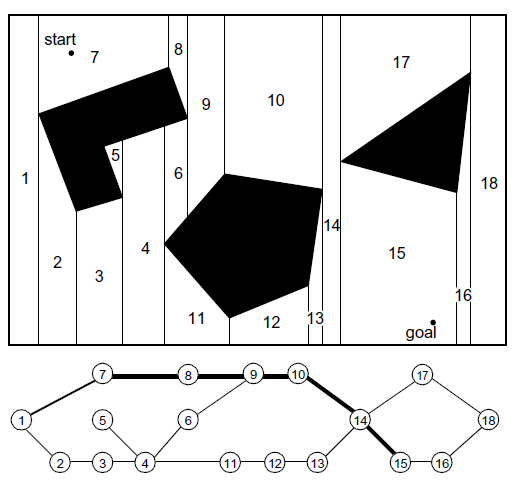
\includegraphics[width=0.7\textwidth]{images/cell_decomposition.png}
	\caption{Exact cell decomposition, 'this image is taken from \cite{Siegwart2004}'.}
	\label{pics:cell_decomposition}
\end{figure}

\section{Potential Field Path Planning}

The idea behind this method is to set up a gradient across the map, such that the robot, represented by a point, is attracted toward the goal, while being repulsed by the obstacles. As one can see in Figure \ref{pics:potential_field}, the resulting field (d) is thus the sum of a attractive (b) and a repulsive potential field (c). This method guides the robot smoothly towards its goal position while avoiding collision with obstacles (e). Potential field path planning can be used in high-dimensional configuration spaces. However, one major drawback of potential fields is the formation of local minima, in where the robot gets trapped. 

\begin{figure} [h]
	\centering
	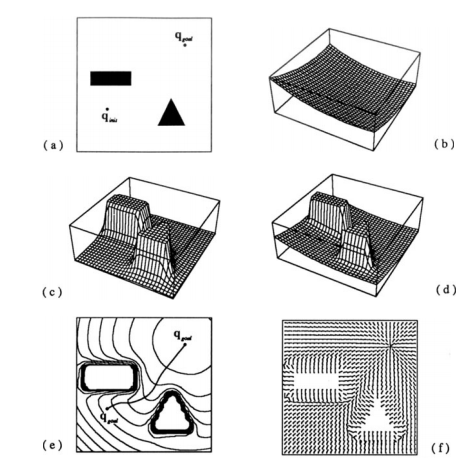
\includegraphics[width=0.9\textwidth]{images/potential_field.png}
	\caption{Different potential fields, 'this image is taken from \cite{Latombe2012}'.}
	\label{pics:potential_field}
\end{figure}

\section{Sampling-Based Algorithms for Path Planning}

These methods are using some form of sampling-based algorithm to produces potential configurations, which are subsequently checked on their feasibility by a collision detector. They can be easily adapted to high-dimensional configuration spaces. One distinguish between multi- and single-query methods. 

\begin{itemize}
	\item
	Multi-query methods are mostly suitable for static environments and consists of a preprocessing phase, where a roadmap is constructed, and a query phase, where a path is planned to connect the start and goal configuration. 
	\item
	In single-query methods, the robot constructs the roadmap while simultaneously searching for a path between initial and goal configuration. Since these methods works online, they are capable for usage in dynamic environments.
\end{itemize}


\subsection{Rapidly-Exploring Random Tree}

RRT (see Figure \ref{pics:rrt}) is a single-query path planning algorithm. It builds a tree of possible configurations that expands from the initial state and tends to cover the whole obstacle-free workspace. At each iteration, a new random node is sampled and the necessary measures are taken to connect it feasible to the tree. A modified version of this algorithm is used for the path planner of this bachelor thesis.

\begin{figure} [h]
	\centering
	\includegraphics[width=0.7\textwidth]{images/rrt.png}
	\caption{RRT tree after (a) 250, (b) 500, (c) 2500 and (d) 10'000 iterations, 'this image is taken from \cite{Karaman2011}'.}
	\label{pics:rrt}
\end{figure} 

\subsection{Probabilistic Roadmap}

Probabilistic roadmap (PRM) (see Figure \ref{pics:prm}) is a multi-query path planning method. In a first step, random samples from the configuration space of the robot are taken. Second, these samples are being checked whether they are located in the free space. In case of being in the obstacle free space, a local planner attempts to connect them to other existing nearby configurations. After the initial and goal states are connected to the constructed roadmap, a graph search algorithm (see also Section ~\ref{sec:graph_search})  is applied to determine a path between both nodes.  

\begin{figure} [h]
	\centering
	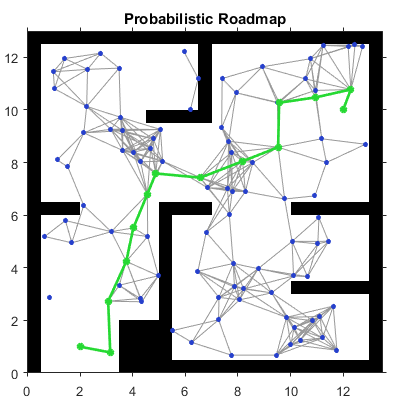
\includegraphics[width=0.7\textwidth]{images/prm.png}
	\caption{An example of a probabilistic roadmap with the path from an initial to a goal configuration marked in green, 'this image is taken from \textit{Mathworks} under the topic Probabilistic Roadmaps'.}
	\label{pics:prm}
\end{figure} 

\section{Graph-Search Algorithms}
\label{sec:graph_search}
This section gives a brief overview of the most common common graph-search algorithms.
\subsection{Lin-Kernighan Heuristic}
The Lin-Kernighan heuristic is an algorithm which deletes existing connections between configurations and reconnects them in other possible ways to generate a more optimal solution. It is commonly used for tasks related to traveling salesman problem\footnote{Searching the shortest route through a list of states.}.

\subsection{Greedy Algorithm}
The Greedy algorithm makes the locally optimal choice at each node. In general, this method does not generate a global optimal sequence of configurations.

\subsection{Label Correcting Algorithm}

With the label correcting algorithm (LCA), the shortest path in a graph network between an initial and a terminal node can be found, assuming the transition cost $a_{ij}$ between state i and j is positive. The algorithm can be summarized in 4 steps (detailed description of the variables and the steps can be found in \cite{Bertsekas1995}): 

\begin{enumerate}
	\item Place the initial node $S$ in the OPEN BIN and set: $d_S=0$ and $d_j=\infty$ $\forall j$ ($d_q$: cost to move from state $S$ to state $q$)
	\item Remove a node $i$ from the OPEN BIN and execute step 3 for all children $j$ of $i$.
	\item If $d_i + a_{ij} < min(d_j, d_T)$ ($d_ {T}$ is the final node), set $d_j = d_i + a_{ij}$ and $i$ to be the parent of $j$. If $j \neq T$, place $j$ in the OPEN BIN if it is not already there. 
	\item If the OPEN BIN is empty, the algorithm is done, else go back to step 1. 
\end{enumerate}

There are multiple options in selecting a node to be removed from the OPEN BIN in step 2, which results in different algorithms:

\begin{itemize}
	\item Depth-first search: Last in, first out. 
	\item Best-first search: Remove best label first (Dijkstra's method). A generalization of this algorithm is A*. By adding a lower bound to the cost function, non-optimal nodes can be excluded.
	\item Breadth-first search: First in, first out (Bellman-Ford). 
\end{itemize}
\cleardoublepage
\chapter{Algorithm Concepts }
\label{sec:algorithm_concepts}

This chapter explains the concepts of the chosen algorithms for the offline global path planner and the path generation around an object in greater detail.

\section{Offline Global Path Planning Algorithm}

RRT* is a variation of the basic rapidly-exploring random tree algorithm as described in \citealp{Karaman2011}. Similiar to its predecessor, the algorithm is able to search high-dimensional configuration spaces by randomly building a tree starting from an initial state. With two further rewiring steps, the algorithm is asymptotically optimal. The following section will consider this offline global path planning algorithm step by step.

\subsection{RRT* Algorithm}
\label{(sec: rrt*)}

In Figure \ref{pics:rrt1}, a partially constructed tree is spreading from a starting configuration into the obstacle-free workspace. Furthermore, a goal state within a specific threshold area is defined. The red circles represent states, which consists of informations
 on their positions. \\

\begin{figure} [h]
	\centering
	\includegraphics[width=1\textwidth]{images/rrt1.png}
	\caption{A new node (black) is being added to the tree.}
	\label{pics:rrt1}
\end{figure}

In a first step, a random state on the map gets sampled. Control is applied from the inherent nearest state to get closer to the sample. In this case, the stepsize is added in the direction of the sample in order to generate a new state. If this connection does not intersect an obstacle, the new state is added to the tree. Otherwise, the current iteration terminates and the process starts from the beginning again by sampling a new configuration. In a further step, new possible parents within a defined neighbourhood radius are considered for the new state. A rewiring is performed, if the new connection is collision-free and results in a path with minimum cost. Thus the current edge gets replaced in order to still maintain a tree structure. Figure \ref{pics:rrt2} shows an example of this process. In Figure \ref{pics:rrt3}, the final rewiring step is taking place. Edges are created from the new state to its possible children vertices, if the path through the new states results in a lower cost than the path through the current parent of the children. At this point, the current iteration is completed and the process starts over again. The procedure is repeated, until a feasible path from the initial to the goal configuration is found (see Figure \ref{pics:rrt4}). Since RRT* is an asymptotically optimal path planning algorithm, this solution gets updated with further iterations.      

\begin{figure} [h]
	\centering
	\includegraphics[width=1\textwidth]{images/rrt2.png}
	\caption{Searching for new parent nodes: a) potential states and b) rewiring  }
	\label{pics:rrt2}
\end{figure}

\begin{figure} [h]
	\centering
	\includegraphics[width=1\textwidth]{images/rrt3.png}
	\caption{Searching for new children nodes: c) potential states and d) rewiring  }
	\label{pics:rrt3}
\end{figure}

\begin{figure} [h]
	\centering
	\includegraphics[width=1\textwidth]{images/rrt4.png}
	\caption{A feasible path between start and goal state.}
	\label{pics:rrt4}
\end{figure}
   
\subsubsection{Search Radius}

The search radius $r_{Search}$ is a non-constant variable and is calculated with the following formula (Formula \ref{eq:radius}):

\begin{equation}
r_{Search} = min(\gamma_{RRT^{*}}(log(card(V))/card(V)^{1/d},\eta)  
\label{eq:radius}
\end{equation}

\begin{equation}
\gamma_{RRT^{*}}>(2(1+1/d))^{1/d}(\mu(X_{free})/\xi)^{1/d}
\label{eq:gamma}
\end{equation}

\begin{itemize}
	\item
	$\gamma_{RRT^{*}}$ is a constant and is chosen such the inequality (Formula \ref{eq:gamma}) is met. On the basis of a theorem, the fulfilment of this requirement results in the asymptotic optimality of the RRT* algorithm,
	\item
	$\mu(X_{free})$ defines the Lebesgue measure\footnote{Measure that associate objects in the euclidean space with their content (length, area, volume)  } of the obstacle-free space,
	\item
	$\xi$ is the volume of the unit sphere\footnote{Sphere with unit radius in d-dimensional space (length, circle, sphere)},
	\item
	$d$ is the dimension of the workspace,
	\item
	$\eta$ corresponds to the stepsize,
	\item
	$card(V)$ defines the current number of configurations available in the workspace.
\end{itemize}

\begin{figure} [h]
	\centering
	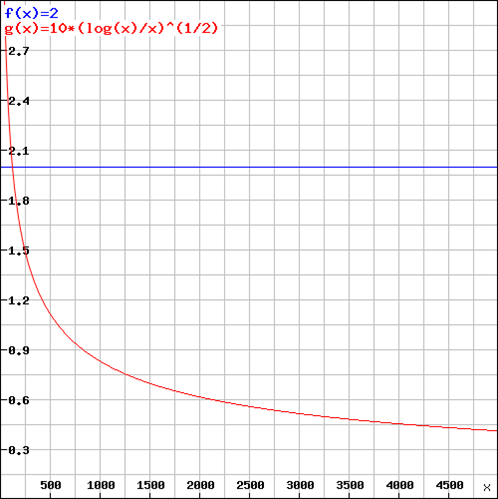
\includegraphics[width=0.75\textwidth]{images/radius.png}
	\caption{Plot of the search radius ($\eta=2,\gamma_{RRT^{*}}=10,d=2$, cardinality on the x- and radius on the y-axis)}
	\label{pics:radius}
\end{figure}

The search radius (see Formula \ref{eq:radius}) decreases logarithmically (see Figure \ref{pics:radius}) with the number of available configuration in the workspace. This choice is logical, since there are less required rewiring in a highly populated map needed. Furthermore, the computational effort of the collision-check function as well as the search of potential neighbours for the rewiring step gets released with a decrease of the search radius, which shortens the overall runtime of the algorithm.   

%\subsubsection{RRT* Pseudocode} 
%
%\begin{algorithm}[H]
%	\SetAlgoLined
%	$V \leftarrow {x_{init}}; E \leftarrow \emptyset$\;
%	\For{$i=1,...,n$}{		
%	$x_{rand} \leftarrow SampleFree$\;
%	$x_{nearest} \leftarrow Nearest(G=(V,E), x_{rand})$ \;
%	$x_{new} \leftarrow Steer(x_{nearest}, x_{rand})$ \; 	
%	\If{ObstacleFree($x_{x_{nearest}}, x_{x_{new}}$)} {
%		$X_{near} \leftarrow Near(G=(V,E), x_{new}, ...$
%		$... min\{\gamma_{RRT^{*}}(log(card(V))/card(V))^{1/d}, \eta)\}$\; 	
%		$V \leftarrow V \cup \{x_{new}\}$\;
%		$x_{min} \leftarrow x_{nearest}; c_{min} \leftarrow Cost(x_{nearest})+c(Line(x_{nearest}, x_{new}))$\;
%		\For{$x_{near} \in X_{near}$}{
%			\If{$CollisionFree(x_{near}, x_{new}) \land Cost(x_{near}) ...$
%			$...+c(Line(x_{near}, x_{new}))<c_{min}$}{
%				$x_{min} \leftarrow x_{near}; c_{min} \leftarrow Cost(x_{near})+c(Line(x_{near},x_{new}))$\;
%				}
%			$E \leftarrow E \cup \{(x_{min},x_{new})\}$\;
%			\For{$x_{near} \in X_{near}$}{
%				\If{$CollisionFree(x_{new}, x_{near}) \land Cost(x_{new})...$
%				$...+c(Line(x_{new}, x_{near})) < Cost(x_{near})$}{
%					$x_{parent} \leftarrow Parent(x_{near})$\;
%					$E \leftarrow (E \backslash \{(x_{parent},x_{near})\}) \cup \{(x_{new},x_{near})\}$\;
%					}			
%				}		
%			}	
%		}	
%	}
%	\textbf{return} $G=(V,E)$\;	
%\end{algorithm}

\section{Path Generation around an Object}

The second goal of the thesis is the generation of a feasible path around an underwater object. Summarized, the process works as follows. 

\begin{itemize}
\item
First N viewpoints around the object are manually calculated,
\item
all possible paths between them are generated,
\item
the order of visiting the viewpoints is figured out.

\end{itemize}

\subsection{Viewpoints Calculation}

The N viewpoints are set, such that the front camera of \textit{Scubo} is able to cover the whole object in one frame. Thus, the distance to the object was estimated with the horizontal and vertical angle of view of the camera. 

\subsection{Paths and Cost Matrix Generation}

In Figure \ref{pics:viewpoints_paths}, the viewpoint 1 is considered first. Feasible paths to other viewpoints are calculated using the RRT* algorithm (see Section \ref{(sec: rrt*)}). The costs, which are defined by the length from one viewpoint to another are stored in a $N\times N$ matrix (see Figure \ref{pics:viewpoints_paths}). 

\begin{figure} [h]
	\centering
	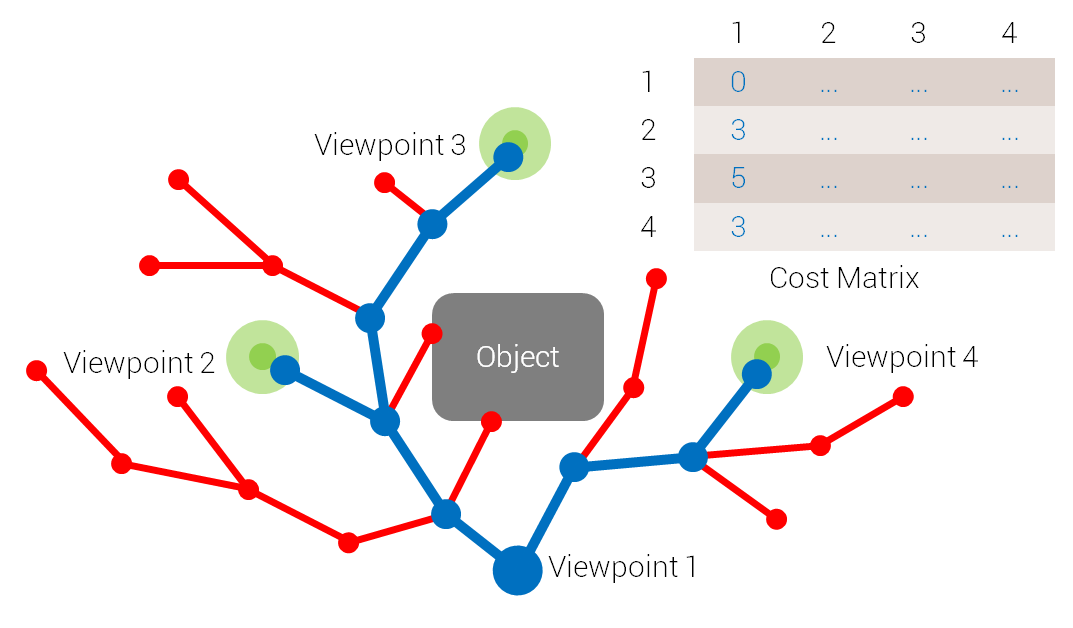
\includegraphics[width=1\textwidth]{images/cost_matrix_and_paths.png}
	\caption{Feasible paths to each viewpoint are calculated with the RRT* algorithm. The length of the paths are stored in a cost matrix.}
	\label{pics:viewpoints_paths}
\end{figure}

\subsection{Traveling Salesman Problem}

With the information about the viewpoints and the costs between them, the task of object scanning is reduced to a traveling salesman problem. The goal is to calculate the shortest possible route that visits each viewpoint exactly once and returns to the starting position. Large amount of heuristic and exact methods are able to approximate a solution of the problem. In the following, two of them are shortly introduced:

\begin{itemize}
	\item
	Greedy Algorithm: Makes the locally optimal choice at each stage. Thus, tends to find a local rather than a global optimum.
	\item
	Lin-Kernighan Heuristic (LKH): Randomly swapping pairs of sub-tours in order to generate a new more cost-optimal tour (see figure \ref{pics:lkh}). 
\end{itemize}

\begin{figure} [h]
	\centering
	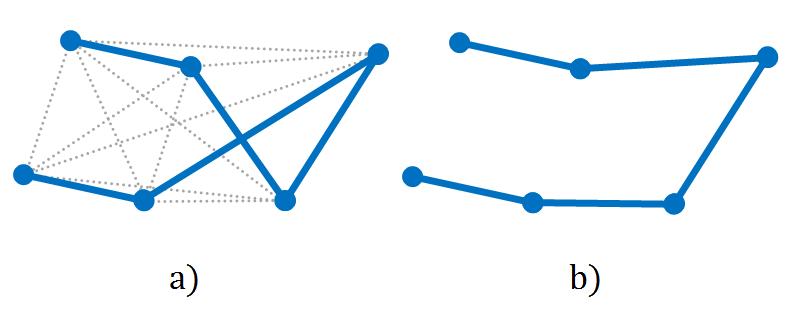
\includegraphics[width=0.6\textwidth]{images/LKH.png}
	\caption{Lin-Kernighan Heuristic: a) possible sub-tours in grey, b) optimal tour through eliminating cross-tours}
	\label{pics:lkh}
\end{figure}
\cleardoublepage
\chapter{Implementation Keypoints }
\label{sec:implementation_keypoints}

This chapter gives an overview of the keypoints regarding the implementation of the methods illustrated in Chapter \ref{sec:algorithm_concepts}.

\section{2D-RRT*}

The RRT* path planner was firstly implemented on a 2D plane. 

\subsection{Runtime Improvement}

The main challenge here was the runtime, which increases exponentially with the number of iterations. As a reference, one of the first implemented versions took approximately 30 minutes to compute 10'000 iterations. This is due to the following reasons:

\begin{itemize}
	\item
	The collision-check function takes two states as an input and scans single points along the connection on collision with a specific check resolution. As one can see in Figure \ref{pics:obstacle_detection}, the smaller the resolution gets, the higher the probability of detecting a potential threat is. However, a small resolution results in long runtime for the collision-check function. Since this function gets called at least once per iteration, it has strong influence on the overall calculation time of the path planner. 
	\item
	At high amount of configurations in the workspace, the search of the nearest neighbour as well as the search of potential neighbours for the rewiring step becomes time-consuming, since the algorithm has to check the distance to each available state one by one.  	
\end{itemize} 

\begin{figure} [h]
	\centering
	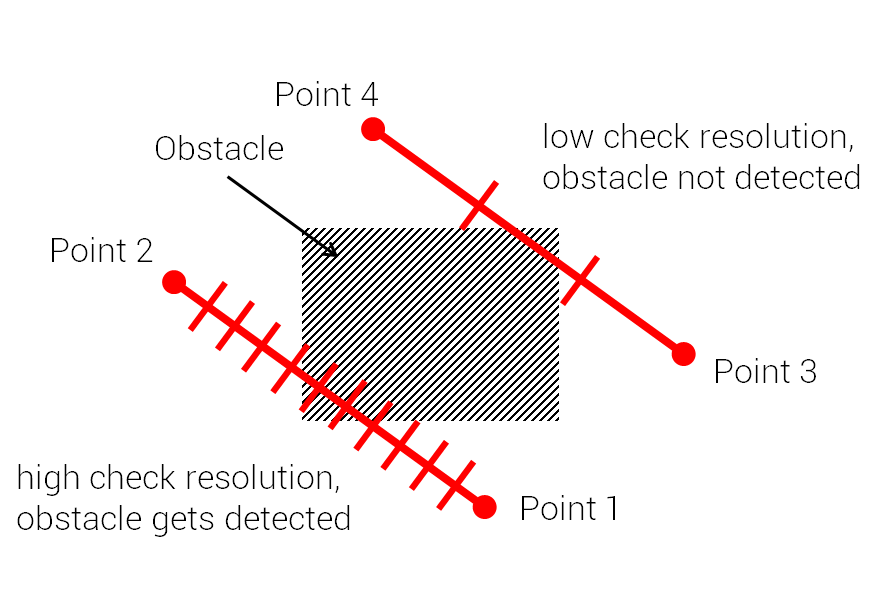
\includegraphics[width=0.75\textwidth]{images/obstacle_detection.png}
	\caption{Influence of the check resolution on obstacle detection.}
	\label{pics:obstacle_detection}
\end{figure}

Both problems can be kept within a limit by the implementation of the variable search radius described in Chapter \ref{(sec: rrt*)}. Regarding the collision-check function, the runtime could be improved by increasing the check resolution. However, this would take place at the expense of safety and is thus not recommendable.\\  

\subsubsection{k-d-tree}

A method called k-dimensional-tree (k-d-tree) can be used to reduce the searching work. It is a data-structure for organizing k-dimensional points by their attributes. As in the example of Figure \ref{pics:kd_tree}, the idea is to divide the configuration space into smaller subgroups. This is done by repeatedly splitting the space at the median of different attributes, which can be represented by a tree. By arrival of a new point, it only needs to be sorted based on its attributes into the corresponding subgroup. This way, the search can be restricted and the runtime improved. This method is an approximating technique and in some cases, errors in the search of the nearest neighbour can occur. In \textit{MATLAB}, k-d-tree is already implemented in the Statistics and Machine Learning Toolbox\footnote{http://ch.mathworks.com/help/stats/index.html}.

 
\begin{figure} [h]
	\centering
	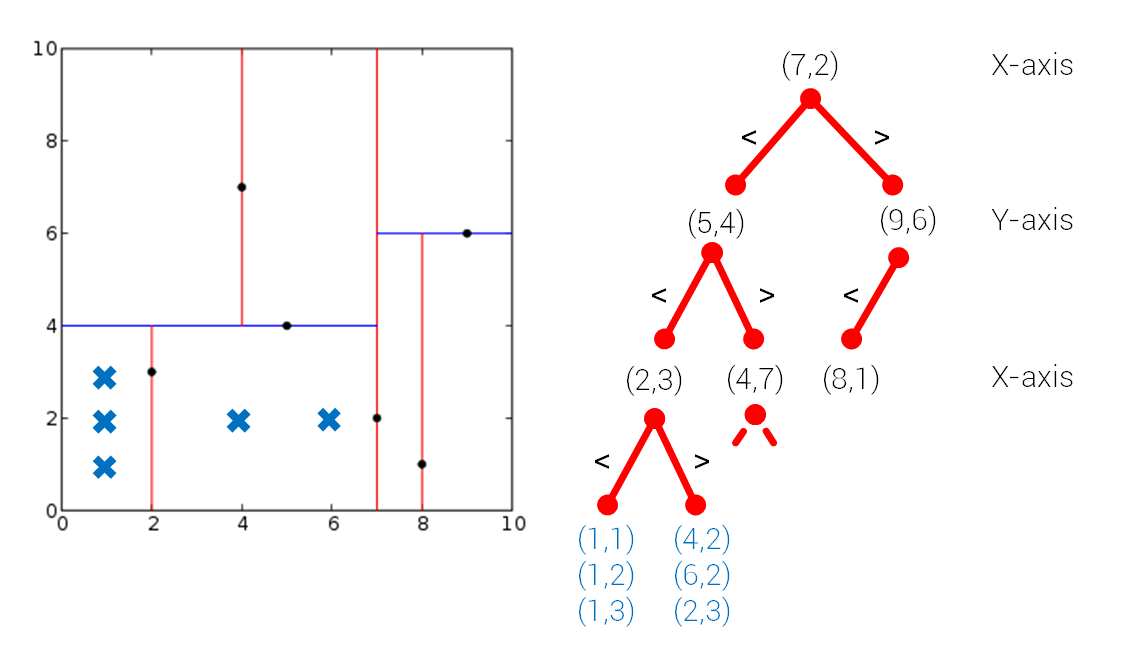
\includegraphics[width=1\textwidth]{images/kd-tree.png}
	\caption{Example of a 2-d-tree.}
	\label{pics:kd_tree}
\end{figure}

\subsubsection{Matrix Operation}

Since \textit{MATLAB} is designed for numerical calculation using matrices, the run time can be minimized by using matrix operations instead of for-loops. In the following, two code parts are shown which shows the search for the nearest state (see Code \ref{matrix_op1}) and the neighbours (see Code \ref{matrix_op2}). Furthermore, a runtime test showed that matrix operations is slightly more time-efficient at high iteration number than k-d-tree (see figure \ref{pics:runtime}).

\begin{figure} [h]
	\centering
	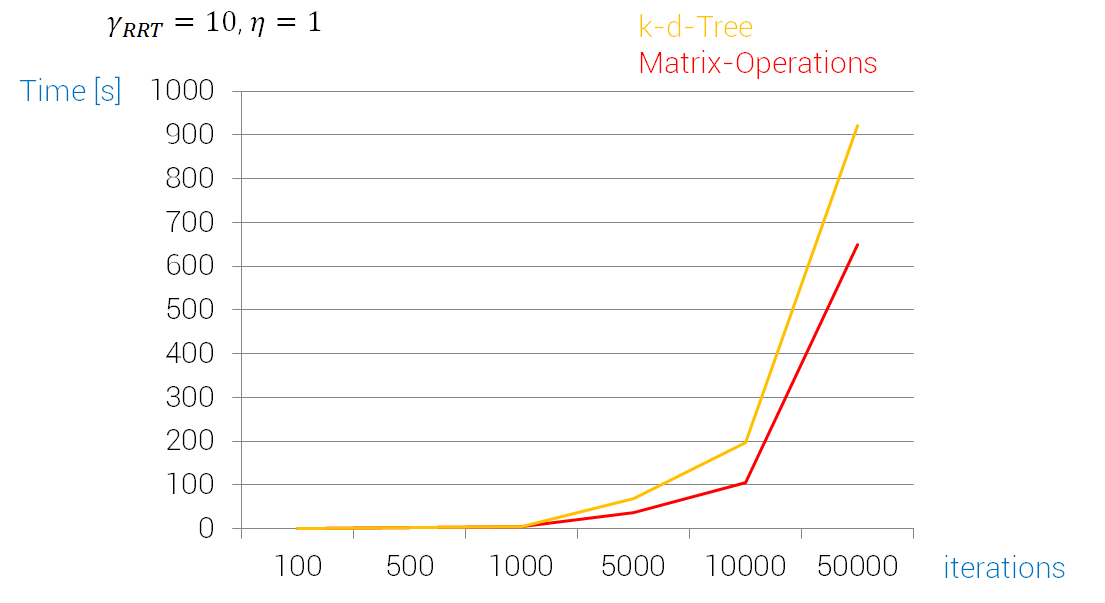
\includegraphics[width=1\textwidth]{images/runtime.png}
	\caption{Calculation time: k-d-tree and Matrix Operations in comparison}
	\label{pics:runtime}
\end{figure}

\begin{lstlisting}[caption={Nearest State Search},label=matrix_op1]
difference_array=states_array(:,1:2)-repmat([x_sample,y_sample],size(states_array,1),1);

distance_array=sqrt(sum(difference_array.^2,2));

[~,idx]=ismember(min(distance_array),distance_array);
\end{lstlisting}

\begin{lstlisting}[caption={Neighbours Search},label=matrix_op2]
distance_array=states_array(:,1:2)-repmat([states_array(i,1),states_array(i,2)],size(states_array,1),1);
        
distance_from_neighbor=sqrt(sum(distance_array.^2,2));
        
neighbors=find(distance_from_neighbor<=search_radius);
\end{lstlisting}

\subsection{Path Curvature}

In a further step, the influence of the cost function on the curvature of the path was evaluated. Both, the euclidean distance as well as the angular change between line segments were considered with corresponding weight-factors in the step cost function (see formula \ref{eq:cost_function}). The angle between two connections were considered in square in order to penalize large angular changes.

\begin{figure} [h]
	\centering
	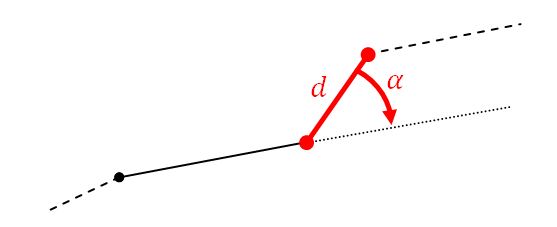
\includegraphics[width=0.6\textwidth]{images/angle.png}
	\caption{Angle $\alpha$ between two connections and distance d.}
	\label{pics:angle}
\end{figure}

\begin{equation}
cost_{step} = w_{1}\,d+w_{2} \,\alpha^{2}
\label{eq:cost_function}
\end{equation} 

\section{3D-RRT*}

The implemented algorithms and functions for the 2D plane was adapted for the 3D configuration space. The main problem was the implementation of a 3D occupancy grid, which will be illustrated in the following section.    

\subsection{3D Occupancy Grid}
Since \textit{Octomap}\footnote{3D mapping framework based on octrees.} does not exist for \textit{MATLAB} and there were no other 3D occupancy grid implementation in the form of a toolbox, the main challenge in the 3D configuration space was the development of a function to differentiate between free and occupied areas. Furthermore, it should be able to use a point cloud (see Figure \ref{pics:pointcloud}) as an input to generate a discretized obstacle model for the planner.\\

\begin{figure} [h]
	\centering
	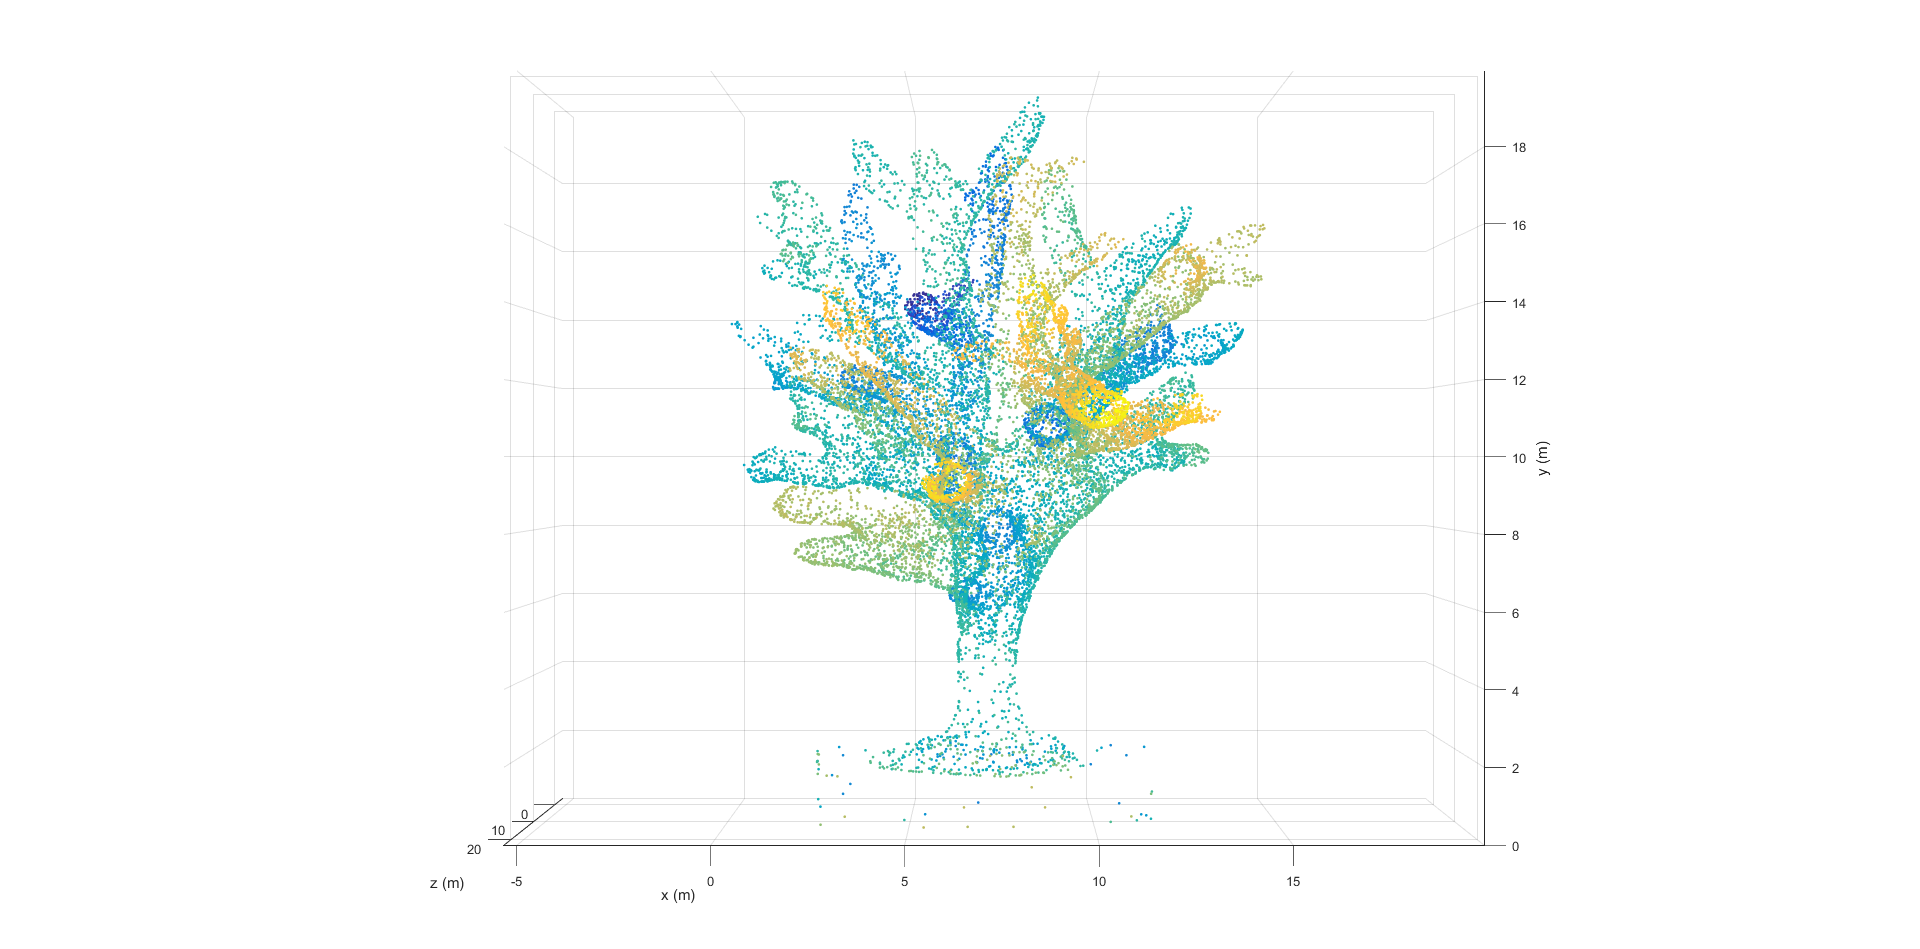
\includegraphics[width=1\textwidth]{images/pointcloud.png}
	\caption{Pointcloud model of a coral.}
	\label{pics:pointcloud}
\end{figure}

\subsubsection{Visualization}
The visualization of the discretized model was done in two steps. The whole configuration space was divided with a certain resolution into single cubical cells. Cells which are occupied by at least one data point from the point cloud were highlighted.    

\begin{figure} [h]
	\centering
	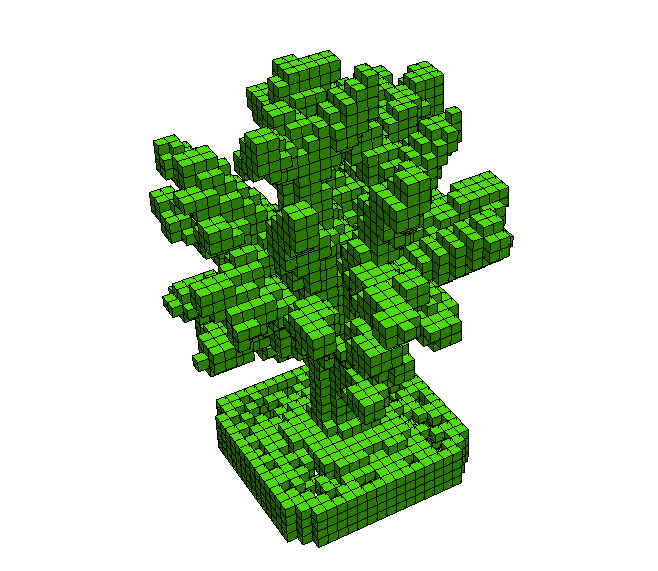
\includegraphics[width=0.5\textwidth]{images/discretized.png}
	\caption{Discretized model of the coral.}
	\label{pics:discretized}
\end{figure}

\subsubsection{Collision-Check}
For collision-checking, the workspace was transformed into a three dimensional matrix according Formulas \ref{eq:occupancy} to \ref{eq:transformation_occupancy}. The size corresponds to the number of cells in the configuration space. Obstacle-free cells carry the value 0 while occupied cells the value 1. 

\begin{equation}
occupancy=zeros(m_{length}/b_{res},m_{width}/b_{res},m_{height}/b_{res})
\label{eq:occupancy}
\end{equation} 

\begin{equation}
[x_{occ},y_{occ},z_{occ}]=[ceil(x_{PC}/b_{res}),ceil(y_{PC}/b_{res}),ceil(z_{PC}/b_{res})]
\label{eq:transformation}
\end{equation}

\begin{equation}
occupancy(x_{occ},y_{occ},z_{occ})=1
\label{eq:transformation_occupancy}
\end{equation} 

\begin{itemize}
	\item
	$m_{length},\,m_{width}$ and $m_{height}$ are the map sizes,
	\item
	$x_{PC},\,y_{PC}$ and $z_{PC}$ are the datapoints from the point cloud,
	\item
	$b_{res}$ is the map resolution respectively the length of a single cubical cell.
\end{itemize}

\section{Object Scanning Route}

The implemented algorithm was used for an object scanning application. For this, the sampling function needed to be rewritten in order to generate solutions within a short amount of time. 

\subsection{Defined Sampling Region}

The RRT* algorithm is not able to generate a feasible paths between all viewpoints (see Figure \ref{pics:viewpoints_paths}) within a relatively short period of time and with a fixed iteration number. This problem was solved by rewriting the sampling function. Instead of sampling in the whole map, the new function samples with 50\% in the goal region (see Figure \ref{pics:sampling}). Therefore, a path is more likely to be found. Furthermore, the program is defined as such that it automatically terminates when all feasible paths are generated. 

\begin{figure} [h]
	\centering
	\includegraphics[width=1\textwidth]{images/sampling_regions.png}
	\caption{Defined sampling region.}
	\label{pics:sampling}
\end{figure}

\cleardoublepage
\chapter{Results}
\label{sec:results}
The results of the developed algorithms will be presented in this chapter. The mentioned programs and functions can be found on the provided CD.   

\section{RRT* Path Planning in 2D}

In this section, the results of the path curvature evaluation on the 2D plane are discussed. In the cost function, one considers euclidean distances on the one hand and angular changes on the other. A cost function consisting of a combination of both attributes does not bring any benefits and therefore was not considered. The m-file \verb+RRTstar_Obstacles_2D.m+ in the folder \verb|Curvature_Evaluation| is used and the following parameters are chosen:

\begin{itemize}
	\item
	$10 \times 9.5$ map
	\item
	$x_{initial}=4.75$ and $y_{initial}=2.75$
	\item
	$x_{initial\_parent}=5$ and $y_{initial\_parent}=2.75$ \footnote{These additional variables are needed to define the heading in the initial configuration}
	\item
	$x_{final}=4.75$ and $y_{final}=6.75$ 
	\item 
	$\gamma_{RRT^{*}}=10$
	\item
	$\eta=1$
	\item
	$iteration=50'000$
\end{itemize} 

\subsection{Cost Function: Considering Euclidean Distance}
\label{sec:euclidean}

\begin{itemize}
	\item
	$w_{1}=1$ and $w_{2}=0$
	\item
	$140\,s$ to complete the calculation.
\end{itemize} 

As one can see in Figure \ref{pics:RRTstar_w1}, the RRT* algorithm calculates a path, which follows mostly the edges of the obstacles. By inflating the obstacles in the order of the radius of \textit{Scubo}, one can create buffer zones for the robot to move without hitting obstacles. Furthermore, the path takes sharp turns at edges. This is also not a problem for the real system, since the robot is omnidirectional and is able to move in any direction without prior change of its orientation.

\begin{figure} [h]
	\centering
	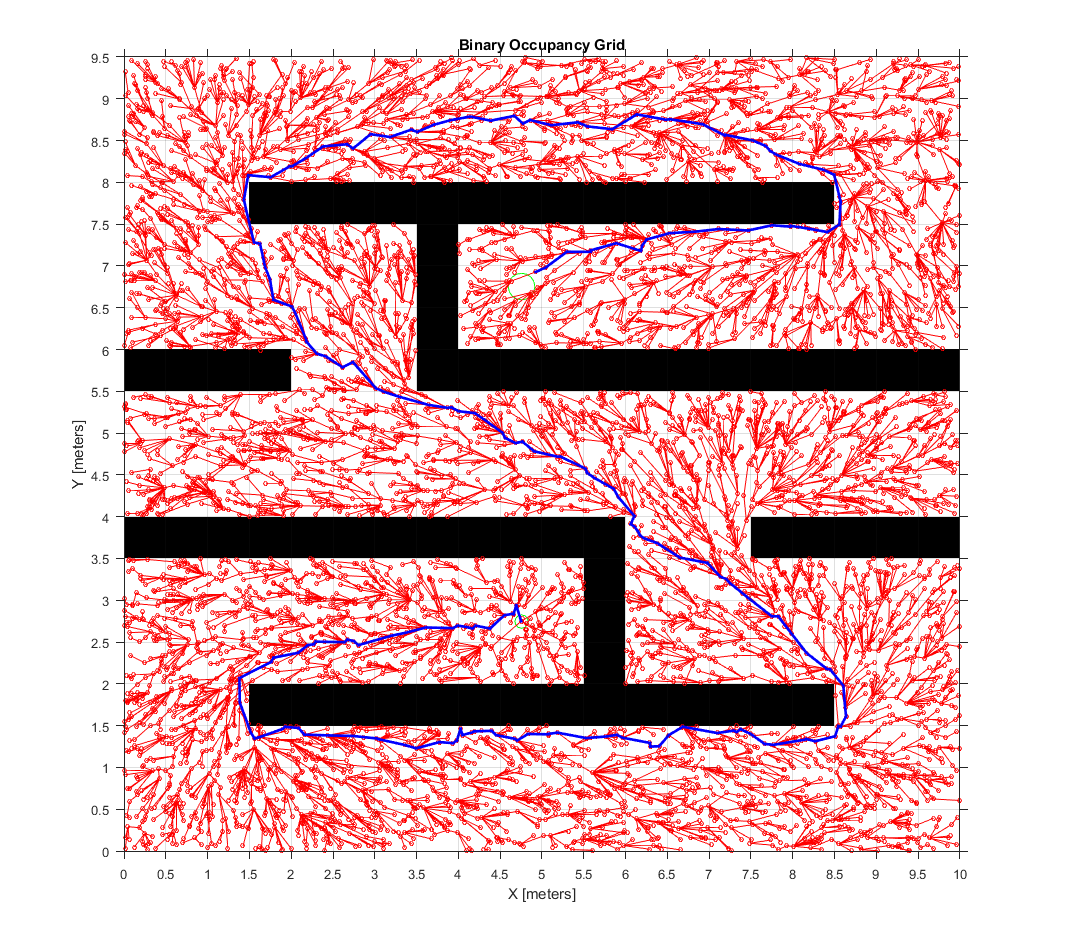
\includegraphics[width=1\textwidth]{images/RRTstar_w1.png}
	\caption{2D RRT* Path: Considering euclidean distance in the cost function.}
	\label{pics:RRTstar_w1}
\end{figure}


\subsection{Cost Function: Considering Angular Change}

\begin{itemize}
	\item
	$w_{1}=0$ and $w_{2}=1$
	\item
	$102\,s$ to complete the calculation.
\end{itemize}

As expected, a much smoother path can be generated under the same condition by considering the angular change in the cost function (see Figure  \ref{pics:RRTstar_w2}). Surprisingly, this task takes less time to compute than the one described in the previous Section  \ref{sec:euclidean}.

\begin{figure} [h]
	\centering
	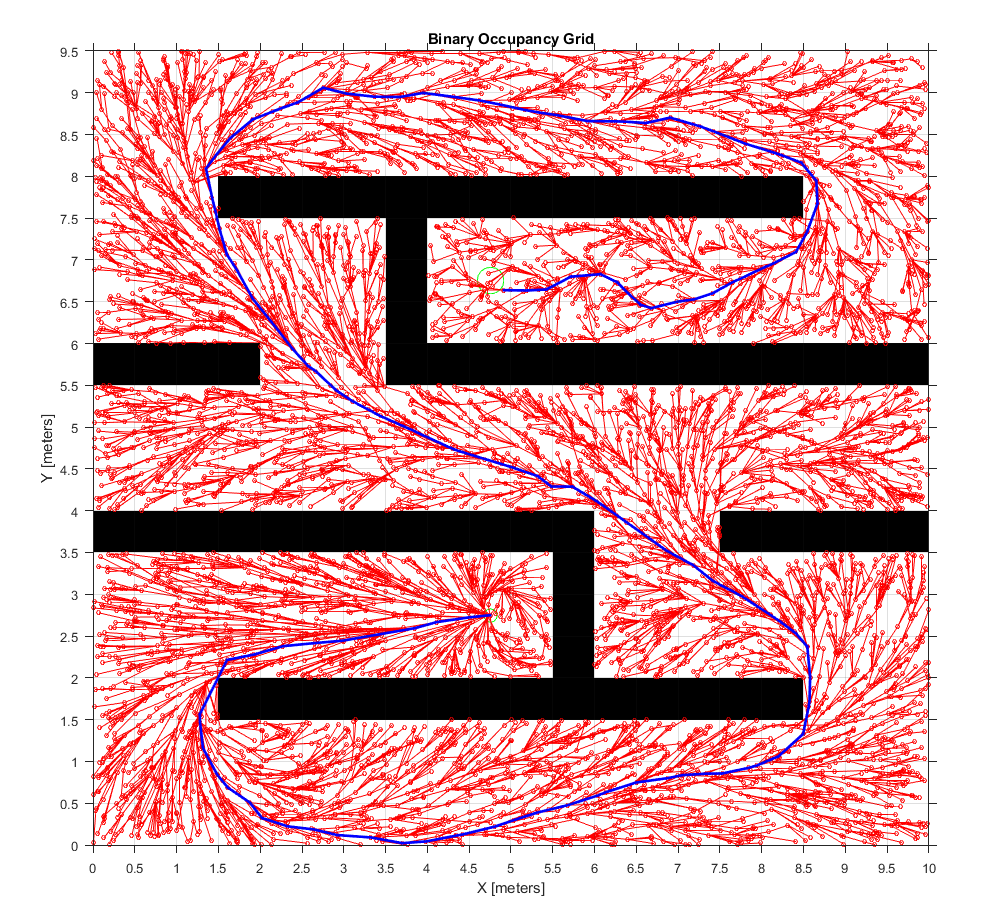
\includegraphics[width=1\textwidth]{images/RRTstar_w2.png}
	\caption{2D RRT* Path: Considering angular change in the cost function.}
	\label{pics:RRTstar_w2}
\end{figure}

\section{RRT* Path Planning in 3D}

The visualization in 3D is done with \textit{Paraview}. The m-file \verb+RRTstar_Obstacles_3D.m+ is used to generate the map, the states and the resulting paths. With \verb+VtkWriter.m+, the results are transformed into VTK-format in order to display it in \textit{Paraview}. The following parameters are chosen:

\begin{itemize}
	\item
	$10 \times 10 \times 10$ map
	\item
	$x_{initial}=1$, $y_{initial}=1$ and $z_{initial}=1$
	\item
	$x_{final}=1$, $y_{final}=1$ and $z_{final}=9$
	\item 
	$\gamma_{RRT^{*}}=10$
	\item
	$\eta=2$
	\item
	$iteration=1000$
\end{itemize}

As one can see in Figure \ref{pics:rrstar_3d}, the generated path in 3D is feasible. The red wall is an obstacle with a hole in the middle. The algorithm is able to find a path between start and goal through the obstacle.

\begin{figure} [h]
	\centering
	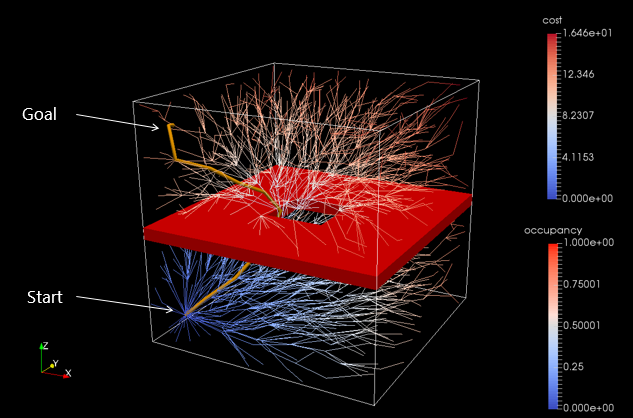
\includegraphics[width=1\textwidth]{images/rrtstar_3d.png}
	\caption{3D RRT* Path}
	\label{pics:rrstar_3d}
\end{figure}

\section{Object Scanning}
\label{sec:object_scanning}

For object scanning, the following files were used. Point cloud datas were stored in \verb+coral.vtr+. The file \verb|occupancy_calculation.m| calculates the occupancy matrix regarding Formulas \ref{eq:occupancy}, \ref{eq:transformation} and \ref{eq:transformation_occupancy}. The viewpoints are set in \verb|view_states_calculation.m| and the corresponding cost matrix and the possible paths between all viewpoints is computed in \verb|traveling_salesman_cost.m|. The order of the viewpoints can be defined in two ways. The file \verb|ts_greedy_algorithm.m| sets the order according the greedy algorithm. For a order by the LKH algorithm, one can use the file \verb|compute_traveling_salesman.m| with the corresponding executables\footnote{http://webhotel4.ruc.dk/~keld/research/LKH/}.  

\subsection{Route by Greedy Algorithm}

As expected, the route generated by the greedy algorithm is not efficient, since the path go over the object two times (see Figure \ref{pics:greedy}).

\begin{figure} [h]
	\centering
	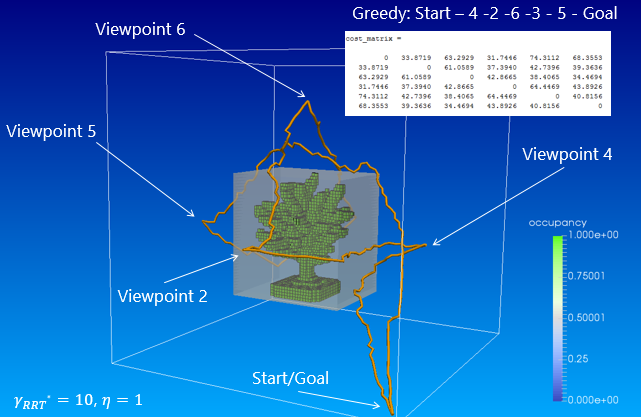
\includegraphics[width=1\textwidth]{images/greedy.png}
	\caption{Object scanning route according greedy algorithm.}
	\label{pics:greedy}
\end{figure}

\subsection{Route by LKH Algorithm}

A much more efficient route can be generated by using the LKH algorithm. The path goes around the object in a reasonable manner and ends in the starting configuration (see Figure \ref{pics:lkh_route}).

\begin{figure} [h]
	\centering
	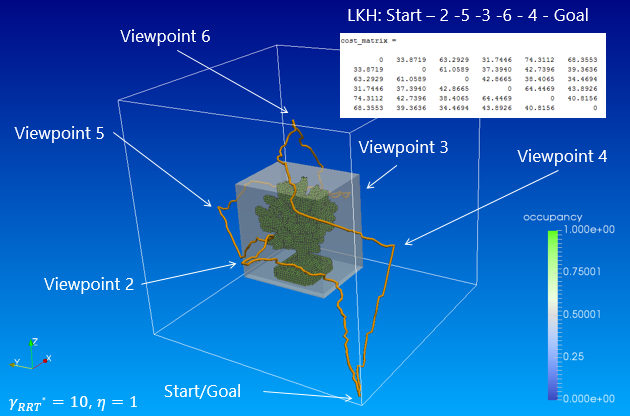
\includegraphics[width=1\textwidth]{images/lkh_route.png}
	\caption{Object scanning route according the LKH algorithm.}
	\label{pics:lkh_route}
\end{figure}
\cleardoublepage
\chapter{Summary}
This chapter gives a brief conclusion of the results and an outlook.

\section{Conclusion}

The RRT* algorithm is proved to be highly suitable for finding paths between two points. In comparison with other methods, it is adaptable to high-dimensional spaces. However, to generate feasible path in large spaces and to get optimal results, long calculation time is required, which is a major drawback of this method. Otherwise, paths, like the one for object scanning (see Section \ref{sec:object_scanning}), would result in a zig-zag-pattern. Although \textit{Scubo} is able to handle such kind of trajectories, they are not pleasing in an efficiency matter.

\section{Outlook}

In a further step, the generated paths need to be smoothed in a post-processing step in order to remove the zig-zag-pattern. Furthermore, the configuration space can be expanded in order to produce a trajectory consisting of position and orientation information. An implementation in C++/ROS and the combination with a trajectory controller is required to test the path planner on the real system. \\

The path planner developed in this bachelor thesis requires information of the static map in order to produce feasible paths from a fixed starting position. However, this rarely the case in real world application. In addition to static, there are also dynamic obstacles. Therefore, an real-time RRT* algorithm in combination with SLAM must be developed in order to recognize moving obstacles and to locally re-plan the path. Additionally, an object identification algorithm must be produced in order to autonomously plan scanning routes. 

   
\cleardoublepage
% \input{}
% \cleardoublepage
% \input{}
% \cleardoublepage
% ...
%

%%%%%%%%%%%%%%%%%%%%%%%%%%%%%%%%%%%%%%%%%%%%%%%%%%%%%%%%%%%%%%%%%%%%%%%%%%%%%%%
% Bibliography
%%%%%%%%%%%%%%%%%%%%%%%%%%%%%%%%%%%%%%%%%%%%%%%%%%%%%%%%%%%%%%%%%%%%%%%%%%%%%%%
\bibliographystyle{bibliography/IEEEtranN}
\bibliography{bibliography/references}
\addcontentsline{toc}{chapter}{Bibliography}
\cleardoublepage

%%%%%%%%%%%%%%%%%%%%%%%%%%%%%%%%%%%%%%%%%%%%%%%%%%%%%%%%%%%%%%%%%%%%%%%%%%%%%%%
% Appendix
%%%%%%%%%%%%%%%%%%%%%%%%%%%%%%%%%%%%%%%%%%%%%%%%%%%%%%%%%%%%%%%%%%%%%%%%%%%%%%%
%\appendix
%\chapter{Irgendwas}\label{sec:irgendwas}

Bla bla \dots
%\cleardoublepage
%\chapter{Datasheets}\label{sec:datasheets}

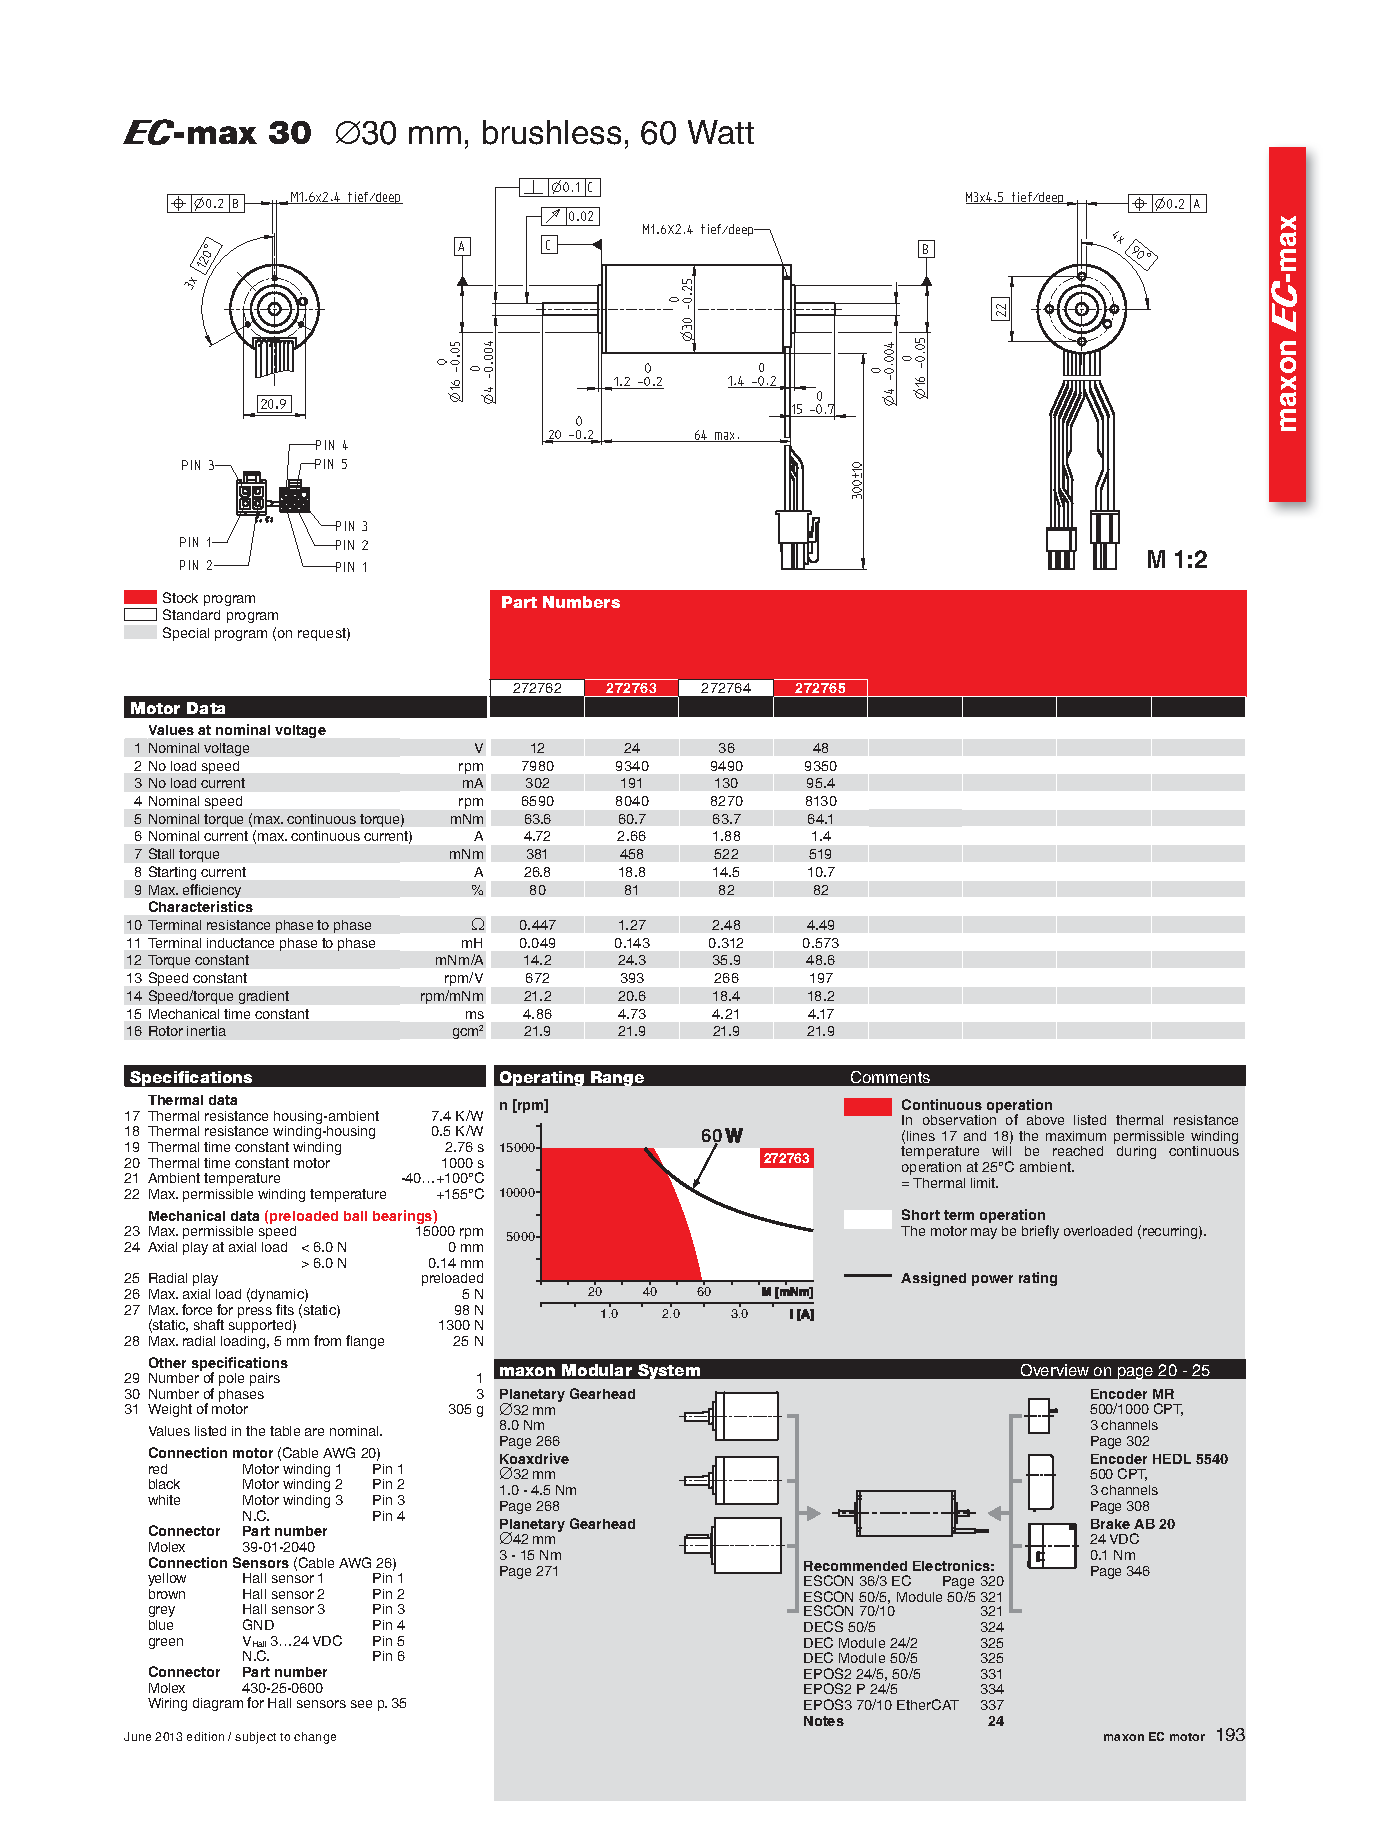
\includepdf[scale=0.75]{images/datasheets.pdf}

\end{document}